\documentclass{ctexbeamer}
\usetheme{Dresden}
\usecolortheme{spruce}
\usepackage{amsmath, amsfonts, amssymb}
\usepackage{tikz}
\usepackage{listings}
\usepackage{xcolor}
\usepackage{underscore}
\usepackage{IEEEtrantools}
\special{dvipdfmx:config z 0} % delete this when release
\usetikzlibrary{positioning, arrows.meta, shapes.geometric}
\title{Processor Arch: Pipelined}
\author{庄嘉毅}
\date{October 2022}

\renewcommand{\footnoterule}{}
\def\QED{\hfill $\square$}
\def\st{\textrm{s.t.}\,}
\def\imply{\draw[-{Implies[]}, double distance=2pt]}
\DeclareMathOperator{\e}{e}
\newcommand{\ftitle}[1]{\frametitle{\hspace{4ex} {#1}}}
\newcommand{\bfig}[2][1.0]{
    \begin{figure}[hb]\centering\resizebox{#1\columnwidth}{!}{#2}
    \end{figure}
}
\newcommand{\roq}[1]{\rotatebox[origin=c]{-90}{#1}}

\setmonofont{Fira Code} 
\lstset{basicstyle=\footnotesize\tt}
\lstset{
    columns=fixed,
    frame=none,                                          % 不显示背景边框
    keywordstyle=\color[RGB]{40,40,255},                 % 设定关键字颜色
    commentstyle=\slshape\color[RGB]{0,96,96},                % 设置代码注释的格式
    stringstyle=\color[RGB]{128,0,0},                    % 设置字符串格式
    showstringspaces=false,                              % 不显示字符串中的空格
    language=c++,                                        % 设置语言
}

\usefonttheme{professionalfonts}
\everymath{\displaystyle}
% \linespread{1.5}

\begin{document}

\begin{frame}
    \titlepage
\end{frame}

\section{为什么需要流水线?}
\begin{frame}
    \ftitle{为什么需要流水线?}

    \begin{itemize}
        \item<2- > 顺序结构无法发挥 CPU 的全部性能.
        \item<3- > 以五阶段处理器为例, 处理器在执行一个阶段时,
            其他阶段的电路都处于空闲状态.
    \end{itemize}

    \onslide<3- >\bfig{
        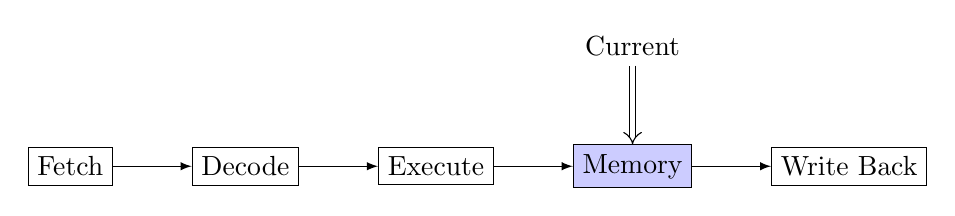
\begin{tikzpicture}
            \node [draw] (A) {Fetch};
            \node [draw, right=of A] (B) {Decode};
            \node [draw, right=of B] (C) {Execute};
            \node [draw, right=of C, fill=blue!20] (D) {Memory};
            \node [draw, right=of D] (E) {Write Back};
            \node [above=of D] (R) {Current};

            \draw[-latex] (A) -- (B);
            \draw[-latex] (B) -- (C);
            \draw[-latex] (C) -- (D);
            \draw[-latex] (D) -- (E);
            \imply (R) -- (D);
        \end{tikzpicture}
    }
\end{frame}

\begin{frame}
    \ftitle{理想的流水线复用}

    \onslide<2- >{每个阶段的电路都在执行一条指令, 如同流水线一样依次进行.}

    \onslide<3- >\bfig{
        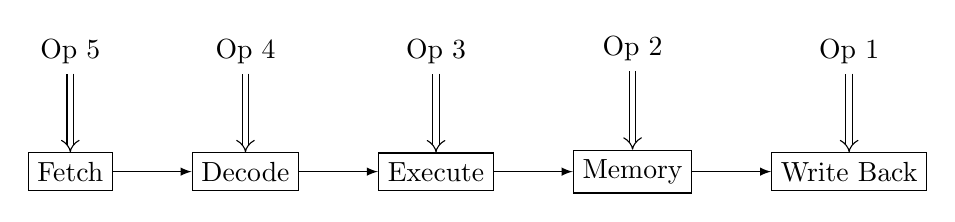
\begin{tikzpicture}
            \node [draw] (A) {Fetch};
            \node [draw, right=of A] (B) {Decode};
            \node [draw, right=of B] (C) {Execute};
            \node [draw, right=of C] (D) {Memory};
            \node [draw, right=of D] (E) {Write Back};
            \node [above=of A] (A1) {Op 5};
            \node [above=of B] (B1) {Op 4};
            \node [above=of C] (C1) {Op 3};
            \node [above=of D] (D1) {Op 2};
            \node [above=of E] (E1) {Op 1};

            \draw[-latex] (A) -- (B);
            \draw[-latex] (B) -- (C);
            \draw[-latex] (C) -- (D);
            \draw[-latex] (D) -- (E);
            \imply (A1) -- (A);
            \imply (B1) -- (B);
            \imply (C1) -- (C);
            \imply (D1) -- (D);
            \imply (E1) -- (E);
        \end{tikzpicture}
    }
\end{frame}

\section{流水线的实现}
\begin{frame}[fragile]
    \ftitle{改造顺序电路}

    \begin{itemize}
        \item<2- > 组合电路与代码不同, 其自身是没有时序保证的.
        \item<4- > 顺序电路的时序是如何保证的?
    \end{itemize}


    \onslide<3- >\begin{columns}
        \begin{column}{.5\linewidth}
            \bfig{
                \begin{tikzpicture}
                    \node (1) at (0, 1) {1};
                    \node (2) at (0, 0) {2};
                    \draw[black] (1, 1.5) rectangle (2, -0.5);
                    \node (ALU) at (1.5, 0.5) {ALU};
                    \draw (1) -- (1, 1);
                    \draw (2) -- (1, 0);
                    \node (3) at (3, 0.5) {3};
                    \draw (2, 0.5) -- (3);
                    \node (4) at (0, -1) {4};
                    \draw[black] (4, 1) rectangle (5, -1.5);
                    \node (ALU) at (4.5, -0.25) {ALU};
                    \draw (3) -- (4, 0.5);
                    \draw (4) -- (4, -1);
                    \node (7) at (6, -0.25) {7};
                    \draw (5, -0.25) -- (7);
                \end{tikzpicture}
            }
        \end{column}
        \begin{column}{.5\linewidth}
            \begin{lstlisting}
int a = 1 + 2;
int b = 4;
int c = a + b;
            \end{lstlisting}
        \end{column}
    \end{columns}
\end{frame}

\begin{frame}
    \ftitle{时序问题}
    \begin{itemize}[<+- >]
        \item 一个逻辑门的输出总是接到另一个逻辑门的输入端.
        \item 电信号传播需要时间, 但无法依赖于此来保证时序.
        \item 在组合逻辑计算完成之后, 如果输入不变, 其状态保持稳定.
        \item 在计算完成之前, 其状态是不稳定的, 不应该使用其结果.
        \item 需要有一个手段来保证稳态是能够对齐的.
    \end{itemize}
\end{frame}

\begin{frame}
    \ftitle{流水线寄存器}
    \begin{itemize}[<+- >]
        \item 寄存器的输出只有收到时钟信号才会改变, 能够起到状态对齐的作用.
        \item 为了在顺序处理器的五个状态之间创造明确的划分,
              需要在每个状态之间加入寄存器.
    \end{itemize}

    \onslide<3- >\bfig{
        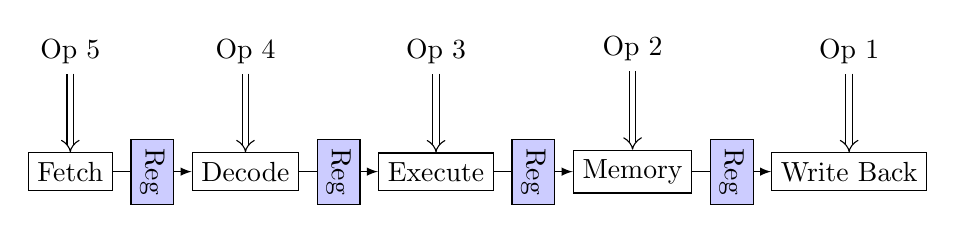
\begin{tikzpicture}
            \node [draw] (A) {Fetch};
            \node [draw, right=of A] (B) {Decode};
            \node [draw, right=of B] (C) {Execute};
            \node [draw, right=of C] (D) {Memory};
            \node [draw, right=of D] (E) {Write Back};
            \node [above=of A] (A1) {Op 5};
            \node [above=of B] (B1) {Op 4};
            \node [above=of C] (C1) {Op 3};
            \node [above=of D] (D1) {Op 2};
            \node [above=of E] (E1) {Op 1};

            \draw[-latex] (A) -- (B) node[midway, draw, fill=blue!20!white] {\roq{Reg}};
            \draw[-latex] (B) -- (C) node[midway, draw, fill=blue!20!white] {\roq{Reg}};
            \draw[-latex] (C) -- (D) node[midway, draw, fill=blue!20!white] {\roq{Reg}};
            \draw[-latex] (D) -- (E) node[midway, draw, fill=blue!20!white] {\roq{Reg}};
            \imply (A1) -- (A);
            \imply (B1) -- (B);
            \imply (C1) -- (C);
            \imply (D1) -- (D);
            \imply (E1) -- (E);
        \end{tikzpicture}
    }
\end{frame}

\begin{frame}
    \ftitle{流水线寄存器}
    \onslide<1- >{顺序相连的寄存器, 形成了逻辑上的队列结构.}

    \foreach \t[evaluate=\t as \p using {int(\t+1)},
        evaluate=\t as \u using {int(\t-1)},
        evaluate=\t as \v using {int(\t-2)},
        evaluate=\t as \w using {int(\t-3)}] in {1,...,4}{
            \onslide<\p- >\bfig[0.8]{
                \begin{tikzpicture}
                    \node [draw, fill=blue!20] (I) at (0, 0) {Inc};
                    \node [draw] (A) at (2, 0) {Reg};
                    \node [draw] (B) at (4, 0) {Reg};
                    \node [draw] (C) at (6, 0) {Reg};
                    \node [draw] (D) at (8, 0) {Reg};
                    \draw[-latex] (I) -- (A) node[midway, above] {\ifnum\t>0 \t \else \fi};
                    \draw[-latex] (A) -- (B) node[midway, above] {\ifnum\u>0 \u \else \fi};
                    \draw[-latex] (B) -- (C) node[midway, above] {\ifnum\v>0 \v \else \fi};
                    \draw[-latex] (C) -- (D) node[midway, above] {\ifnum\w>0 \w \else \fi};
                    \node (E) at (9, 0) {$\cdots$};
                \end{tikzpicture}
            }
        }
\end{frame}

\begin{frame}
    \ftitle{实例:自增电路}
    \onslide<1- >{一个自增电路, 每个时钟周期输出值加1.}
    \onslide<2- >\bfig[0.6]{
        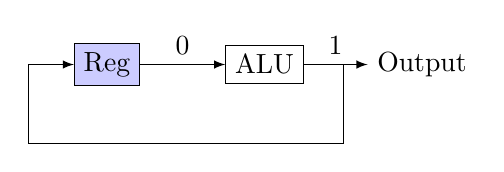
\begin{tikzpicture}
            \node [draw, fill=blue!20] (I) at (0, 0) {Reg};
            \node [draw] (A) at (2, 0) {ALU};
            \node (O) at (4, 0) {Output};
            \draw[-latex] (I) -- (A) node[midway, above] {0};
            \draw[-latex] (A) -- (O) node[midway, above] {1};
            \draw[-latex] (3, 0) -- (3, -1) -- (-1, -1) -- (-1, 0) -- (I.west);
        \end{tikzpicture}
    }

    \onslide<3- >{推广: PC 预测.}

    \onslide<3- >\bfig[0.6]{
        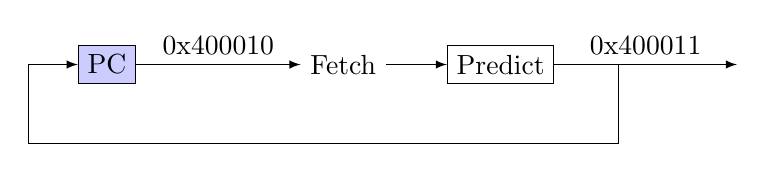
\begin{tikzpicture}
            \node [draw, fill=blue!20] (I) at (0, 0) {PC};
            \node (O) at (3, 0) {Fetch};
            \node [draw] (A) at (5, 0) {Predict};
            \draw[-latex] (I) -- (O) node[midway, above] {0x400010};
            \draw[-latex] (O) -- (A);
            \draw[-latex] (A) -- (8, 0) node[midway, above] {0x400011};
            \draw[-latex] (6.5, 0) -- (6.5, -1) -- (-1, -1) -- (-1, 0) -- (I.west);
        \end{tikzpicture}
    }
\end{frame}

\begin{frame}
    \ftitle{流水线寄存器}
    \begin{itemize}
        \item<1- > 流水线寄存器里面有什么?
            \onslide<2- >\begin{itemize}
                \item 上一个阶段的计算结果.
                \item 之前的阶段接收的值, 没有经过计算, 但会在之后阶段用到.
            \end{itemize}
        \item<3- > 依赖时序的数据连接不会越过流水线寄存器.
    \end{itemize}
\end{frame}

\section{流水线冒险}
\begin{frame}
    \ftitle{流水线冒险}
    \begin{itemize}
        \item<2- > 数据冒险
            \begin{itemize}
                \item<3- > 下一条指令需要某一个寄存器参与运算, 但上一条指令更新了这个寄存器.
            \end{itemize}
        \item<4- > 控制冒险
            \begin{itemize}
                \item<5- > 下一条指令是条件跳转, 需要上一条指令确定条件码.
                \item<6- > 下一条指令是 \texttt{ret}, 需要访问内存确定下一条指令的地址.
            \end{itemize}
    \end{itemize}
\end{frame}

\begin{frame}
    \ftitle{数据转发}
    \begin{itemize}
        \item<2- > 前后两条指令的执行在流水线中相差一个阶段.
        \item<3- > 寄存器数据的读取发生在译码阶段, 此时上一条指令正在执行阶段.
        \item<4- > 如果寄存器的新值在执行阶段时就能够计算出来
            (例如 \texttt{add} 这样的算数指令),
            那么就可以把结果直接传递给下一条指令.
        \item<5- > 如果寄存器的新值在执行阶段得不到
            (例如 \texttt{movq (\%rsp), \%rax}),
            则无法进行数据转发.
    \end{itemize}
\end{frame}

\begin{frame}
    \ftitle{分支预测}
    \begin{itemize}
        \item<2- > 对于 \texttt{jxx} 指令, 倾向于认为条件成立.
            \begin{itemize}
                \item<3- > 其他跳转策略: 向低地址跳转.
                \item<4- > 原理: 大量的条件跳转发生在循环中, 而循环在未结束时往往向低地址跳转.
            \end{itemize}
        \item<5- > 对于 \texttt{ret} 指令, 可以使用硬件栈进行预测, 或者放弃预测.
    \end{itemize}
\end{frame}

\begin{frame}
    \ftitle{暂停与取消}
    \begin{itemize}
        \item<2- > 发生加载/使用冒险而暂停时, 关闭PC寄存器和译码寄存器的写入,
            向执行寄存器写入 \texttt{bubble}/\texttt{nop}.
            \begin{itemize}
                \item<3- > 关闭写入: 使电路不断重复执行同一条指令的某个阶段.
            \end{itemize}
        \item<4- > 遇到 \texttt{ret} 指令而暂停时, 之后的三个周期里,
            取值阶段的行为改为直接向译码寄存器写入 \texttt{bubble}/\texttt{nop}.
        \item<5- > 发生取消时, 向译码和执行寄存器写入 \texttt{bubble}/\texttt{nop}.
            \begin{itemize}
                \item<6- > 不需要关闭寄存器写入, 因为这两种情况都在等待新的PC.
            \end{itemize}
    \end{itemize}
\end{frame}

\begin{frame}
    \ftitle{异常处理}
    \begin{itemize}
        \item<2- > 异常发生后, 需要保证异常指令之前的指令能继续走完流水线,
            同时避免异常指令之后的指令的副作用.
        \item<3- > 流水线寄存器中的 \texttt{stat} 状态位用于标记异常.
        \item<4- > \texttt{stat} 走出流水线时, 实际引发异常.
        \item<5- > \texttt{stat} 在流水线内时, 屏蔽其之后的指令的副作用(访存/写回/条件码).
    \end{itemize}
\end{frame}

\section{性能分析}
\begin{frame}
    \ftitle{吞吐率}
    \begin{itemize}
        \item<2- >$\mathrm{CPI}$: 每指令周期数.
        \item<2- >$\mathrm{IPC}$: 每周期指令数.
        \item<2- >$\mathrm{GIPS}$: 每秒十亿指令数.
    \end{itemize}

    \onslide<3- >\begin{align*}
        \mathrm{CPI}   & = \frac{C_i+C_b}{C_i} = 1 + \frac{C_b}{C_i}    \\
        \onslide<4- >{ & = 1 + \mathrm{lp} + \mathrm{mp} + \mathrm{rp}}
    \end{align*}

    \onslide<4- >$\mathrm{lp}$: 加载/使用惩罚;
    $\mathrm{mp}$: 分支预测错误惩罚;
    $\mathrm{rp}$: \texttt{ret}指令惩罚.

\end{frame}

\begin{frame}
    \ftitle{性能分析}

    \onslide<1- >插入 2 个流水线寄存器, 使得运行时间最短.
    假设寄存器的读写延迟为 20ps.

    \only<1>{\bfig[0.8]{
            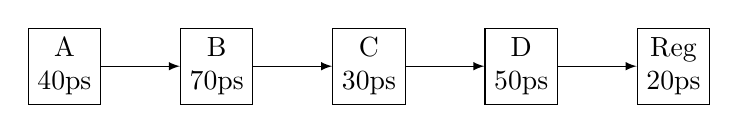
\begin{tikzpicture}
                \node [draw, align=center] (A) {A\\40ps};
                \node [draw, right=of A, align=center] (B) {B\\70ps};
                \node [draw, right=of B, align=center] (C) {C\\30ps};
                \node [draw, right=of C, align=center] (D) {D\\50ps};
                \node [draw, right=of D, align=center] (E) {Reg\\20ps};


                \draw[-latex] (A) -- (B);
                \draw[-latex] (B) -- (C);
                \draw[-latex] (C) -- (D);
                \draw[-latex] (D) -- (E);
            \end{tikzpicture}
        }}

    \only<2- >{\bfig[0.8]{
            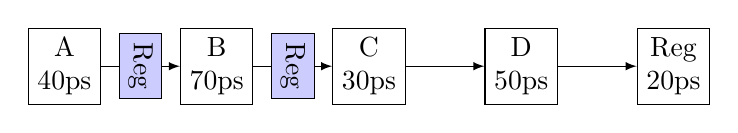
\begin{tikzpicture}
                \node [draw, align=center] (A) {A\\40ps};
                \node [draw, right=of A, align=center] (B) {B\\70ps};
                \node [draw, right=of B, align=center] (C) {C\\30ps};
                \node [draw, right=of C, align=center] (D) {D\\50ps};
                \node [draw, right=of D, align=center] (E) {Reg\\20ps};


                \draw[-latex] (A) -- (B) node[midway, draw, fill=blue!20!white] {\roq{Reg}};
                \draw[-latex] (B) -- (C) node[midway, draw, fill=blue!20!white] {\roq{Reg}};
                \draw[-latex] (C) -- (D);
                \draw[-latex] (D) -- (E);
            \end{tikzpicture}
        }}

    \onslide<3- > 计算吞吐率($\mathrm{GIPS}$).

    \onslide<4- >\begin{gather*}
        \mathrm{GIPS} = 1 \mathrm{s}/((30+50+20)\times 10^{-12}\mathrm{s})\times 10^{-9} = 10.00
    \end{gather*}
\end{frame}

\section{拓展内容}
\begin{frame}[fragile]
    \ftitle{乱序执行}
    \begin{itemize}
        \item<2- > 超标量: 每个时钟周期可以进行多个操作.
        \item<2- > 乱序执行: 指令可以不按照程序顺序执行.
        \item<3- > 用更加复杂的控制器(ICU)和执行器(EU)代替流水线结构.
            ICU 可以在一个时钟周期内读取多条指令,
            EU 拥有多个执行单元, 并且同一功能可以有多个执行单元执行.
        \item<4- > 现代PC处理器基本都使用乱序执行的架构.
    \end{itemize}

    \onslide<5- >\begin{lstlisting}
mrmovq  -0x8(%rbp), %rax
addq    %rax, %rdx          # no need stalling
subq    %r8, %rcx
addq    %rcx, %rdx
    \end{lstlisting}
\end{frame}

\begin{frame}
    \ftitle{指令重排序}
    \begin{itemize}
        \item<2- > 指令重排序: 为了提高性能, 编译器会对指令进行重排序,
            减少相邻指令之间的依赖关系.
        \item<3- > 与 CPU 乱序执行不同, 编译器可以实现更大窗口的重排序.
        \item<4- > 通过充分的指令重排序, 流水线处理器可以达到乱序执行 85\% 以上的性能\footnotemark.
    \end{itemize}

    \footnotetext<4- >{\scriptsize McFarlin D S, Tucker C, Zilles C. Discerning the dominant out-of-order performance advantage: Is it speculation or dynamism?[J]. ACM SIGARCH Computer Architecture News, 2013, 41(1): 241-252.}
\end{frame}

\begin{frame}[fragile]
    \ftitle{指令重排序}
    一般来说, 指令重排序不应该改变程序的行为.
    \onslide<2- >\begin{columns}
        \begin{column}{.5\linewidth}
            \begin{lstlisting}[language=c++]
/* before reordering */
int curr = *next;

int value = arr[curr];
do_task(value);

*next = curr + 1;
            \end{lstlisting}
        \end{column}
        \begin{column}{.5\linewidth}
            \begin{lstlisting}[language=c++]
/* after reordering */
int curr = *next;

*next = curr + 1;

int value = arr[curr];
do_task(value);
            \end{lstlisting}
        \end{column}
    \end{columns}

    \onslide<3- > 这种重排序有可能改变程序的行为吗?
\end{frame}

\begin{frame}[fragile]
    \ftitle{内存屏障}
    在并行程序中, 有可能会因为重排序导致错误的行为.

    \onslide<2- >\begin{columns}
        \begin{column}{.5\linewidth}
            \begin{lstlisting}[language=c++]
/* writer */
int curr = *next;
*next = curr + 1;

int value = arr[curr];
do_task(value);
            \end{lstlisting}
        \end{column}
        \begin{column}{.5\linewidth}
            \begin{lstlisting}[language=c++]
/* reader */
int curr = *next;

if (curr >= n+1) {
    printf("%d done", n);
}
            \end{lstlisting}
        \end{column}
    \end{columns}

    \begin{itemize}
        \item<3- > 当 \texttt{next} 为 \texttt{n+1} 时,
            其他线程会认为任务 \texttt{n} 已经完成,
            但重排序后的代码无法保证这一行为.
        \item<4- > 由于并行产生的重排序副作用是编译器无法预料的.
    \end{itemize}
\end{frame}

\begin{frame}[fragile]
    \ftitle{内存屏障}
    \onslide<1- > 内存屏障: 用于限制编译器和 CPU 的指令重排序,
    保证程序的行为不会改变.
    \onslide<2- >\begin{lstlisting}[language=c++]
/* writer */
int curr = next.load(std::memory_order_consume);
next.store(curr + 1, std::memory_order_release);
int value = arr[curr];
do_task(value);
/* reader */
int curr = next.load(std::memory_order_acquire);
if (curr >= n+1) {
    printf("%d done", n);
}
    \end{lstlisting}
\end{frame}

\begin{frame}
    \ftitle{内存屏障}
    常见的内存屏障:
    \begin{itemize}
        \item<1- > gcc 拓展: \texttt{__asm__ __volatile__("" ::: "memory")};
        \item<2- > x86_64 指令: \texttt{mfence}, \texttt{lfence};
        \item<3- > 原子变量(C++11/Rust): \texttt{std::atomic<T>}.
    \end{itemize}
\end{frame}

\end{document}
